
\section{Implementation}
	\subsection{Style Guide}
		\subsubsection{Indentation, Line length and Whitespace}
			Use tabs, not spaces, for indentation. Set tabs to equal four spaces.\\Braces should appear on the line below their preceding argument, indented to the same level. All code contained within the braces should be indented by one additional tab. The contents of $<$php? ?$>$ tags should always be indented. The contents of HTML and JavaScript tags may or may not be indented depending on their scope. For example, in HTML the contents of a $<$div$>$ should be indented while the contents of a $<$p$>$ should not. In JavaScript, the contents of a $<$form$>$ should be indented while the contents of an $<$option$>$ should not. The properties of a CSS selector should be indented.\\Line length should not exceed 85 characters. When using HTML $<$p$>$ tags to display text, the contents of the paragraph do not need to comply with line length limits. If the line exceeds 85 characters, the $<$/p$>$ tag should be placed on the line below the textual content of the paragraph.\\Methods containing more than 30 lines of code are discouraged. If a method is over 30 lines of code, it can probably be written more efficiently and/or broken down into multiple methods.\\Readability is a priority over small file sizes; use of whitespace is encouraged where appropriate.
			
		\subsubsection{Naming Conventions}
		Filenames should not contain capital letters. Underscores are only used for pages that pass information from the client to the server. These pages should have a shared, meaningful name followed by \_form or \_post to indicate whether the page is collecting information (\_form) or processing information (\_post).\\CSS specifications should not contain capital letters or underscores. Use of dashes is discouraged, though it is allowed if appropriate. ID and class names should refer to the contents rather than the appearance of an element. For example, "errormsg" is preferable to "smallredtext" in the interests of maintainability.\\Variable names in PHP and JavaScript should use camel casing. The names of boolean variables should begin with "is."
			
		\subsubsection{Structure of Pages}
			All displayable pages on the VirPong website will begin and end with PHP tags to include the header and footer.\\All textual content will be placed within HTML $<$p$>$ tags, with the exception of headers which will be within the header tag of the appropriate level (e.g. $<$h1$>$).\\All HTML and CSS code will comply with the W3C validators in an effort to maximize cross-browser compatibility.
			
		\subsubsection{Documentation Conventions}
			HTML comments should be formatted like so:\\$<$!-- This is a comment. --$>$\\CSS, PHP, and Javascript comments may be formatted in either of the following two ways:\\/**\\* This is a comment. Generally used at the beginning of a block of code to explain\\* its overall function in plain English.\\*/\\or\\// This is a comment. Generally used within blocks of code to explain how certain\\// elements are being used. Generally does not take up more than one line -- if you\\// have that much to say, consider a block comment.
			
		\subsubsection{HTML Specific}
			All HTML tags and attributes will be entirely in lowercase.\\All opening HTML tags will be accompanied by a corresponding closing tag. When using multiple tags, all elements will be properly nested (e.g. $<$b$>$$<$i$>$text$<$/i$>$$<$/b$>$ rather than $<$b$>$$<$i$>$text$<$/b$>$$<$/i$>$). All singleton tags will be closed with a space and an ending slash at the end of the tag (e.g. $<$br /$>$).\\Attributes inside of HTML tags should be contained within double quotes. There should be no spaces between the attribute, the equals sign, and the definition. When defining multiple attributes, they should be separated by a single space.\\All image tags will contain an alt attribute.\\Div layers are generally preferable to tables and iframes. Divs will be used to display the main site layout. Tables should only be used in select cases, such as to display the contents of the database. Iframes should never be used.
			
		\subsubsection{CSS Specific}
			All CSS will be contained in the external stylesheet rather than included as inline style.\\When defining styles for specific elements, think carefully about whether the selector should be an ID or a class. Elements that are only used once on each page (e.g. the content div) should use IDs; elements that may be repeated (e.g. the errormsg) should use classes.\\All text sizes should be specified using ems, not pixels.
			
		\subsubsection{PHP Specific}
			Control statements (if, for, while, switch, etc.) should have one space between the control keyword and the opening parenthesis, to distinguish them from function calls.\\Long if statements may be split onto several lines to comply with line length limits. The conditions should be indented by one additional tab with the logical operators (e.g. \&\&) at the beginning of the line. The first condition may be indented to align with the others. The closing parenthesis and opening brace get their own line at the end of the conditions.\\Literal strings should be contained within singled quotes. When a literal string contains apostrophes, it should instead be contained within double quotes. SQL statements may be contained within double quotes whether or not they contain apostrophes.\\String concatenation will be done using the "." operator with spaces on both sides. When string concatenation exceeds line length limits, the statement should be broken up such each successive line begins with the "." operator aligned under the initial "=" operator.
			
		\subsubsection{JavaScript Specific}
			Any JavaScript code that defines functions should be kept in an external .js file.
			
		\subsubsection{Sources}
			http://na.isobar.com/standards/\\
			http://pear.php.net/manual/en/standards.php
			
	\subsection{Installation}
		There are a few requirements to installing and using our application. Our development platform is Ubuntu and the following are requirements for the installation:
		\begin{description}
			\item[Install a LAMP Server] A LAMP server is composed of a Linux environment, and installations of Apache, MySQL and PHP. However, this step is outside the scope of our tutorial, but you may follow this guide:\\ 
		http://www.howtoforge.com/ubuntu\_debian\_lamp\_server
			\item[Install git] Both our application and Node.js are hosted on git, so it is important to install git on your machine. Installation of git will be covered in the next requirement
			\item[Install Node.js] This is how we are going to run our Javascript on the server. You can follow these directions here to install Node.js:\\http://howtonode.org/how-to-install-nodejs
			\item[Install NPM] NPM is a package manager and has become the standard for installing node libraries. We are going to use this to install socket.io, and you can install NPM by entering the following command in your terminal window 'curl http://npmjs.org/install.sh | sh'
			\item[Install Socket.io] This is how we are going to create bidirectional communication between the server and browser. To install, enter the following command in your terminal window: 'npm install socket.io'
		\end{description}
		Prior to installing the VirPong web application, the database needs to be configured to match the database used with the VirPong game. Once the MySQL database is installed, do the following:
		\begin{enumerate}
			\item Log into your MySQL database. From your terminal window:
			\begin{enumerate}
				\item enter 'mysql -u $<$your\_username$>$ -p'
				\item press enter
				\item enter '$<$your\_password$>$'
				\item press enter
			\end{enumerate}
			\item Now that you're logged into MySQL, the database needs to be created. From the MySQL prompt, enter the following command:\\'CREATE DATABASE db2'
			\item This creates the database, but tables must be created within the database. To create the three tables that are used in the VirPong game, enter the following three commands into the MySQL prompt
			\begin{enumerate}
				\item create table GamesPlayed (gameID INT(10) NOT NULL AUTO\_INCREMENT, username1 VARCHAR(50) NOT NULL, username2 VARCHAR(50) NOT NULL, score1 TINYINT NOT NULL, score2 TINYINT NOT NULL, win TINYINT NOT NULL, INDEX index1(gameID), CONSTRAINT FK\_customer FOREIGN KEY(username1) REFERENCES customer(username), CONSTRAINT FK\_customer\_2 FOREIGN KEY(username2) REFERENCES customer(username));
				\item create table Customer (username VARCHAR(50) NOT NULL, password VARCHAR(50) NOT NULL, firstname VARCHAR(50) NOT NULL, lastname VARCHAR(50) NOT NULL, email VARCHAR(256) NOT NULL, birthday DATE NULL, gender TINYINT NULL, PRIMARY KEY(username));
				\item create table Registration (gameID INT NOT NULL AUTO\_INCREMENT, username1 VARCHAR(50) NOT NULL, username2 VARCHAR(50) NOT NULL, gameTime DATETIME NOT NULL, tournamentID INT NULL,  INDEX index1(gameID), CONSTRAINT FK\_customer FOREIGN KEY(username1) REFERENCES customer(username), CONSTRAINT FK\_customer\_2 FOREIGN KEY(username2) REFERENCES customer(username));
			\end{enumerate}
			\item With all three tables created, exit the MySQL prompt to continue the installation process, by entering:\\'exit'
		\end{enumerate}
		With all of the requirements installed as well as the MySQL database, we can begin running the application. To get the source code for our application:
		\begin{enumerate}
			\item Navigate in your terminal window to your Apache root folder (by default, this is /var/www):\\'cd /./var/www'
			\item Clone our source code by issuing the following command in your terminal window:\\'git clone git://github.com/VirPong/human-pong.git'
			\item Navigate to into the Communication folder:\\'cd human-pong/WebUI/site/http/communication'
			\item Run the VirPong web server by issuing command in your terminal window:\\'node server.js'\\Note: The client.js code may need to be changed depending on your system configuration. Simply change open the client.js file and change the IP address to the address of your server. ex: 'socket = io.connect('xxx.xxx.xxx.xxx');' With your server's address in the parenthesis
			\item To view the application in use, point your web browser to: 'http://localhost/human-pong/WebUI/site/http/communication/index.html'
		\end{enumerate}
		To incorporate this HTML file into your own application, simply follow the steps above and create a link from your website to the Live Game page by making a link in your HTML file to the index.html file.\\To find further instructions on how to install the VirPong platform, or to find other resources that pertain to VirPong, please visit our repository and wiki page at: https://github.com/VirPong/human-pong
		
	\section{Design Patterns}
		\subsection{Pattern Name - Home Link}
		\begin{description}
		\item[Intent] To always provide the user with a simple path to the website's home page.
		\item[Implementation] The VirPong logo in the upper left corner of the layout is a hyperlink to the VirPong home page. This is present on every page.
		\item[Consequences] Allows users to navigate to the home page no matter what page they start at. This is especially helpful if users arrive at the website via a search engine or an emailed link to a specific page.
		\item[Related Patterns] Main Navigation, Footer Bar
		\item[Pattern Name] Main Navigation
		\item[Intent] To always provide the user with hyperlinks to all areas of the website.
		\item[Implementation] The horizontal bar at the top of the layout is a menu containing dropdowns with links to different pages of the VirPong website. This is present on every page.
		\item[Consequences] Allows users to navigate to a page of their choosing no matter what page they start at.
		\item[Related Patterns] Home Link, Footer Bar
	\end{description}
	\subsection{Pattern Name - Footer Bar}
	\begin{description}
\item[Intent] To always provide the user with hyperlinks to important informational content regarding the use of the system.
\item[Implementation] The centered bar at the bottom of the layout is a footer containing links to important information regarding the services that VirPong provides. These links are: about us, contact us, privacy policy, terms of use, and code of conduct. This is present on every page.
\item[Consequences] Allows users to directly access information about the service no matter what page they start at.
\item[Related Patterns] Home Link, Main Navigation
\end{description}
\subsection{Pattern Name - Account Registration}
\begin{description}
\item[Intent] To only display protected content to users who have registered with the service. To store user information which can later be used to enhance the user experience.
\item[Implementation] Users must fill out the registration form before they can play VirPong games, participate in tournaments, or use the chat feature.
\item[Consequences] Allows for personalization of the VirPong experience, including display of personal player history information, the ability to chat with other users, email notifications regarding tournament participation, and happy birthday emails. Trade-offs include potential loss of users who are discouraged by the registration form.
\item[Related Patterns] Lazy Registration, Log In, Input Feedback
\end{description}
\subsection{Pattern Name - Lazy Registration}
\begin{description}
\item[Intent] To allow users to become familiar with the service before requiring them to register.
\item[Implementation] Users can watch VirPong matches (both live and past matches) and view high score information without being registered or signed in to an account. Users can also access all informational content (about us, contact us, privacy policy, terms of use, code of conduct, rules, system requirements, news) without being registered or signed in to an account.
\item[Consequences] Allows users to try out the system with little immediate commitment, making registration seem like more of a choice than a chore. Allows users to be already invested in VirPong by the time they register for an account, making it more likely that our registered users are active uses. Trade-offs include potential loss of registered accounts by users who only utilize features that do no require registration.
\item[Related Patterns] Account Registration
\end{description}
\subsection{Pattern Name - Log In}
\begin{description}
\item[Intent] To identify a registered user in order to properly personalize their experience.
\item[Implementation] The main navigation contains a link to the log in form, allowing registered users to authenticate into the system whenever they desire. If an unauthenticated user attempts to access a page that is only available to registered users, it will display a prompt asking the user to log in before proceeding.
\item[Consequences] Allows for personalization of the VirPong experience, including unlocking access to certain pages that are only available to registered users.
\item[Related Patterns] Account Registration
\end{description}
\subsection{Pattern Name - Input Feedback}
\begin{description}
\item[Intent] To communicate with users about information they are submitting to the service.
\item[Implementation] All improperly filled out forms will generate specific error messages, whether through Javascript alerts or inline text. All properly filled out forms will lead to a success message, confirming that the user�s submission was successful. This design pattern applies to the registration, log in, and account settings forms.
\item[Consequences] Prevents improper information submission by alerting the user immediately and directly of any errors. Allows the user to feel confident upon receipt of success message that their information has been passed to the system.
\item[Related Patterns] Account Registration, Good Defaults
\end{description}
\subsection{Pattern Name - Good Defaults}
\begin{description}
\item[Intent] To prevent users from having to type any more keystrokes than strictly necessary by prefilling certain form values to anticipate the user input.
\item[Implementation] The account settings form automatically fills in the user�s current first name, last name, email address, birthday, and gender. The user can then edit any fields he wants to change and leave any fields he wants to remain the same.
\item[Consequences] Eliminates the need for the user to reenter all of their information in order to change any field, resulting in significantly increased convenience for the user. Trade-offs include reminding users that we have their personal information and we know how to use it.
\item[Related Patterns] Input Feedback
\end{description}


	\section{Data Storage}
		Within the website's database, we have established three different classes of information that we will be storing: information provided by the client that is related to the world outside of VirPong, information specified by the client that will identify the client within the VirPong world, and information recorded about game play or game statistics. Among the information in the personal class, is their full name, their email address, their birthday, and their gender. Our website's database second class stores information that is unique to our clients and is just as sensitive as their personal information. Among this class of information is our client�s username, their password, the games that they have played, and the times that they have played these games at. The rest of the data that we store in the website's database makes up a third class of information, information that pertains to VirPong games. The data associated with this class includes unique game ID's, the game times, and scores of games, and who won a specific game. Although we have three specific classes of data that we are storing, some of the data exists in multiple classes, such as the times that users have played games, and their specified username and passwords.

\subsection{ER Diagram}
	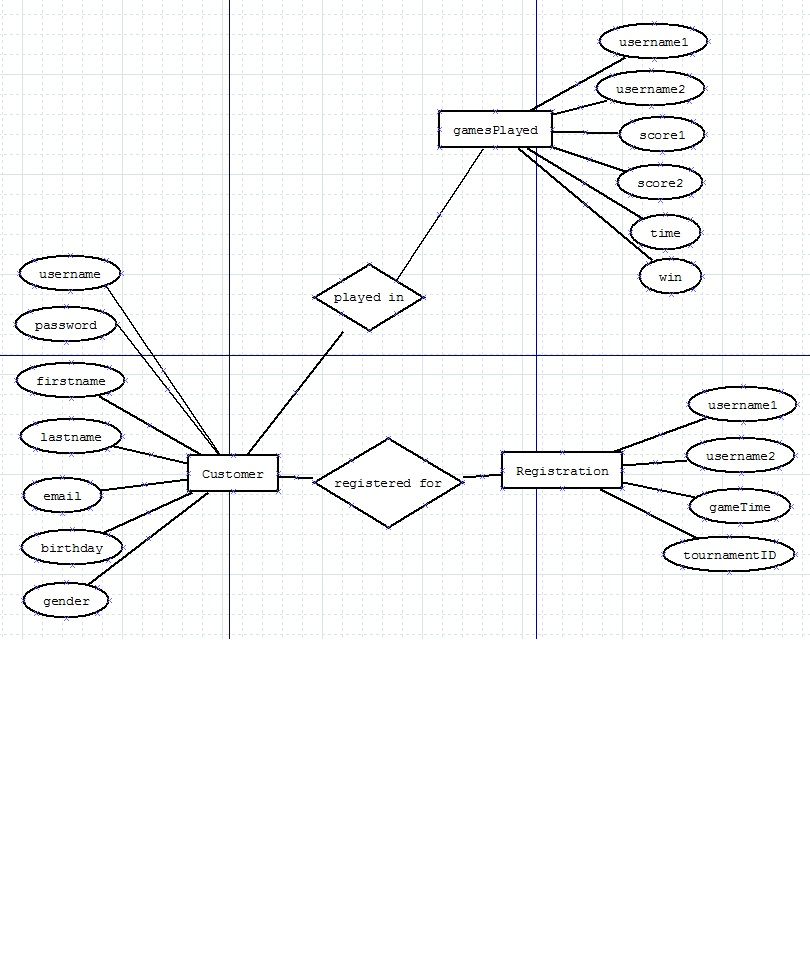
\includegraphics[width=1.0\textwidth]{./ER.jpg}

\newpage

\subsection{Database Schema:}
\begin{description}
\item[Table:] Customer twice

\begin{center}
    \begin{tabular}{ | l | l | l | l | l | l|}
    \hline
    Field & Type & Null & Key & Default & Extra \\ \hline \hline
    username & varchar(50) & NO & PRI & NULL & \hspace{1 pc} \\ \hline
    password & varchar(50) & NO & \hspace{1 pc} & NULL &\hspace{1 pc}  \\ \hline
    firstname & varchar(50) & NO & \hspace{1 pc}& NULL &\hspace{1 pc}  \\ \hline
    lastname & varchar(50) & NO &\hspace{1 pc} & NULL &\hspace{1 pc}  \\ \hline
    email & varchar(256) & NO &\hspace{1 pc} & NULL &\hspace{1 pc}   \\\hline
    birthday & date & YES &\hspace{1 pc} & NULL & \hspace{1 pc} \\ \hline
    gender & tinyint(4) & YES &\hspace{1 pc} & NULL &\hspace{1 pc}  \\
    \hline
    \end{tabular}
\end{center}

    \item[username:] This is the primary key for the Customer database and therefore cannot be null. This will store the user names specified by our customers.
    \item[password:] This field stores the password for the customer. This field cannot be null because it is important for us to maintain the ability to authenticate all users.
    \item[firstname:] This field stores the user�s first name. This field cannot be null because we would like to identify our users by sending them personal messages.
    \item[lastname:] This field stores the user�s last name. This field also cannot be null because we would like to also include the last name of our customer in our personal messages.
    \item[email:] This field stores the email address for the user. We will be sending notifications of future games and must have the ability to contact our customers, therefore this field cannot be null.
	\item[birthday:] This field will store the birthday of our customer. This field can be null if the user would like.
	\item[gender:] This field stores the gender of the customer. This field can be null if the user would like.
\end{description}

\begin{description}

\item[Table:] GamesPlayed

\begin{center}
    \begin{tabular}{ | l | l | l | l | l | l|}
    \hline
    Field & Type & Null & Key & Default & Extra \\ \hline \hline
    gameID & int(10) & NO & MUL & NULL & auto\_increment \\ \hline
    username1 & varchar(50) & NO & MUL & NULL &\hspace{1 pc}  \\ \hline
    username2 & varchar(50) & NO & MUL& NULL &\hspace{1 pc}  \\ \hline
    score1 & tinyint(4) & NO &\hspace{1 pc} & NULL &\hspace{1 pc}  \\ \hline
    score2 & tinyint(4) & NO &\hspace{1 pc} & NULL &\hspace{1 pc}   \\\hline
    win & tinyint(4) & NO &\hspace{1 pc} & NULL & \hspace{1 pc} \\
    \hline
    \end{tabular}
\end{center}
\item[gameID:] This is the key for the GamesPlayed table and it allows us to uniquely identify each game played. This field is automatically incremented by the database.
\item[username1:] This stores the user name of one of the customers that played in this match. This will never be null since we know the users that played in the game.
\item[username2:] This stores the user name of one of the customers that played in this match. This will never be null since we know the users that played in the game.
\item[score1:] This will store username1�s final score. This field will not be null since we need to know the player�s scores.
\item[score2:] This will store username2�s final score. This field will not be null since we need to know the player�s scores.
\item[win:] This field will denote the winner, with either a 1 or a 2 depending on the number of the user that won, of the game played.

\end{description}
\begin{description}

\item[Table:] Registration

\begin{center}
    \begin{tabular}{ | l | l | l | l | l | l|}
    \hline
    Field & Type & Null & Key & Default & Extra \\ \hline \hline
    gameID & int(11) & NO & MUL & NULL & auto\_increment \\ \hline
    username1 & varchar(50) & NO & MUL & NULL &\hspace{1 pc}  \\ \hline
    username2 & varchar(50) & NO & MUL& NULL &\hspace{1 pc}  \\ \hline
    gameTime & datetime & NO &\hspace{1 pc} & NULL &\hspace{1 pc}  \\ \hline
    tournamentID & int(11) & YES &\hspace{1 pc} & NULL &\hspace{1 pc}   \\
    \hline
    \end{tabular}
\end{center}

\item[gameID:] This is the key for the Registration table and it allows us to uniquely identify each upcoming game. This field is automatically incremented by the database.
\item[username1:] This stores the user name of one of the customers playing in this match. This will never be null since these are established future game with two users.
\item[username2:] This stores the user name of one of the customers playing in this match. This will never be null since these are established future game with two users.
\item[gameTime:] This field stores the date and time for the future match to occur.
\item[tournamentID:] This field is used to denote whether a game is part of a tournament. By allowing a null value for tournamentID, we are able to show that a game isn�t a tournament game, and when the game is a tournament game, we can specify that it is a tournament game, as well as  which tournament game, by inserting that tournament�s numeric ID.
\end{description}

\textbf{Reasoning for this design choice:}
    We chose to design our database this way so that we have tables that are specific to the role that the tables are playing. We chose this path because we did not want to have all of our data stored in a single table, which would cause inconsistencies in inserting data into the table. The Customer table is created with information that is specific to identifying our client, as well as personal information that will benefit their VirPong experience. The GamesPlayed table contains information about games that have already been played, including the final score of the game, and who won the game. The Registration table contains data about upcoming games.
    In our Customer table, we have elected to store a client�s identifying information such as their first name, last name, and user name. We also store a password, because we want to maintain that people that are logged into our site are registered users. We also store information such as email addresses, to notify our clients of upcoming events or registered games, as well as client birthdays to wish clients happy birthdays. The email field is also 256 characters long, because this is the longest possible length of an email address.
    The Games Played table holds information specific to games that have been played in the past. Within the table, we store the ID of the game that has been played, so we can uniquely identify games. We also store the names of both users so we can display the players in a certain game, as well as the win field, which references the winning player, so we can determine game statistics. The table also stores the score for each player so we can follow the scores of certain players, as well as the scores for an individual game.
    The last table, Registration holds data that is used to plan a game in advance. We use a game ID to uniquely identify the games in question, but also require the use of a Game Time so that we can remind players when a game is upcoming, as well as to have absolute times for when games are to occur. We also store the names of both players, which we can use to reference the Customer table, to send notifications to the players, as well as advertise which players are about to play a game. The last field, the tournament ID is also used to tell whether or not a certain game is part of a tournament. The field allows an input of null, so when a certain game is not part of a tournament, we can specify null.
	
	
	\subsection{Testing and Verification}
		The testing and verification for the VirPong website will be through validators and various kinds of testing. All the HTML and CSS code will be ran through the W3C validators available online. They will check for the indicated doctype syntax compliance of all of our scripts and compare them against the XHTML 1.1 standard. For all other types of scripts we will be using Google’s developer tools in Google Chrome to see resource load times and any errors thrown by the scripts.

We plan on performing four types of testing upon our code: unit, integration, system, and regression. For the unit testing we are going to use a program called QUnit. We will then uses integration testing across multiple departments of code. Then we will do some system testing against all of our requirements. In this stage of testing we will test scripts in the latest versions of Microsoft’s Internet Explorer, Mozilla’s Firefox, Apple’s Safari, and Google’s Chrome on a Windows 7 machine and a Ubuntu distribution of Linux. We will also report on each functionalities success on each platform and browser to report to the user. Lastly we will perform regression testing when we make additional releases of the software to make sure they implement all functions.

\newpage